%%---------------------------------------------------------------------------%%
%% builder classes for imc-dev manual
%%---------------------------------------------------------------------------%%

\section{Builder Model in \imctest}

The builder objects take input from an interface (IT) and build the
necessary objects required for an IMC calculation.

\subsection{Builder Model Design}

The builder classes are shown in Table~\ref{tab:classes}.  The
builders hook directly into the interface module.  The structure of
the builder model is illustrated in Fig.~\ref{fig:builder}.
\begin{figure}
  \begin{center}
    \begin{tabular}{cc}
      \subfigure[Host-topology build model.]{
        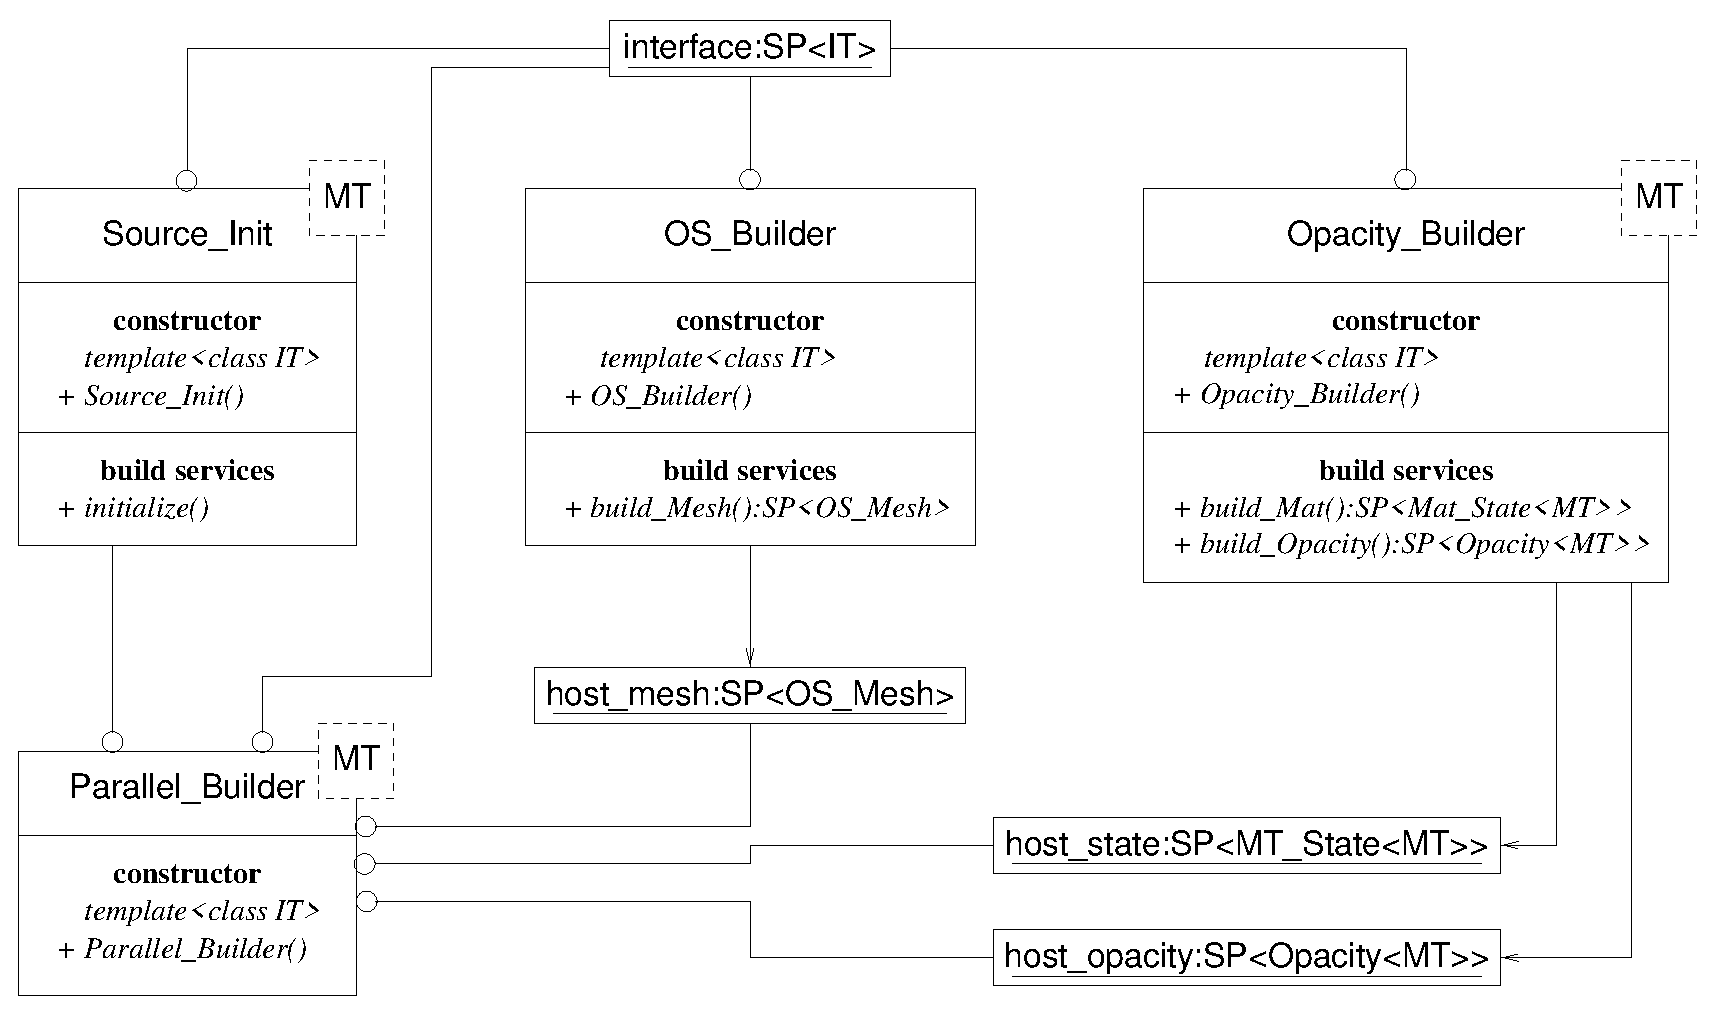
\includegraphics[width=6in]{host_build.eps}} \\
      \subfigure[IMC-topology build model.]{
        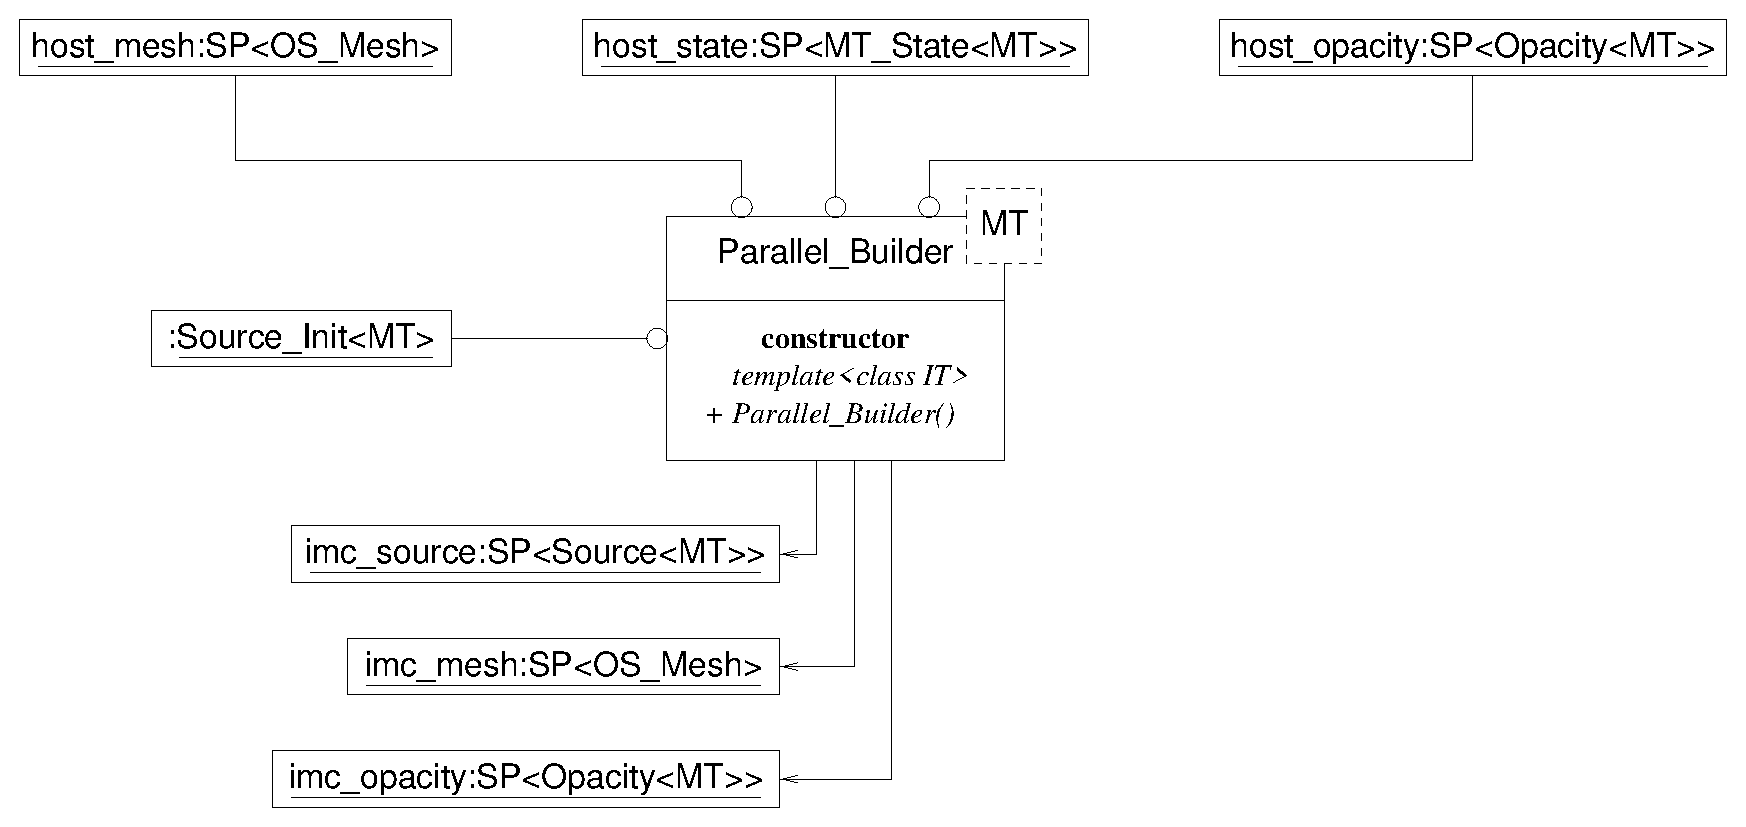
\includegraphics[width=6in]{imc_build.eps}} \\
    \end{tabular}
  \end{center}
  \caption{Builder model featuring the classes described in
    Table~\ref{tab:classes} on the a) host-topology and b)
    IMC-topology.}
  \label{fig:builder}
\end{figure}

\subsection{\comp{OS\_Builder} Class}

The general public interface for \comp{OS\_Builder} is displayed in
Fig.~\ref{os_builder-int}.  \cdFramedFigure{os_builder-int}{Public
  interface for the \comp{OS\_Builder} class.}

\subsection{\comp{Opacity\_Builder} Class}
 
The general public interface for \comp{Opacity\_Builder} is displayed
in Fig.~\ref{opacity_builder-int}.
\cdFramedFigure{opacity_builder-int}{Public interface for the
  \comp{Opacity\_Builder} class.}

